
		\tikzset{every picture/.style={line width=0.75pt}} %set default line width to 0.75pt        

	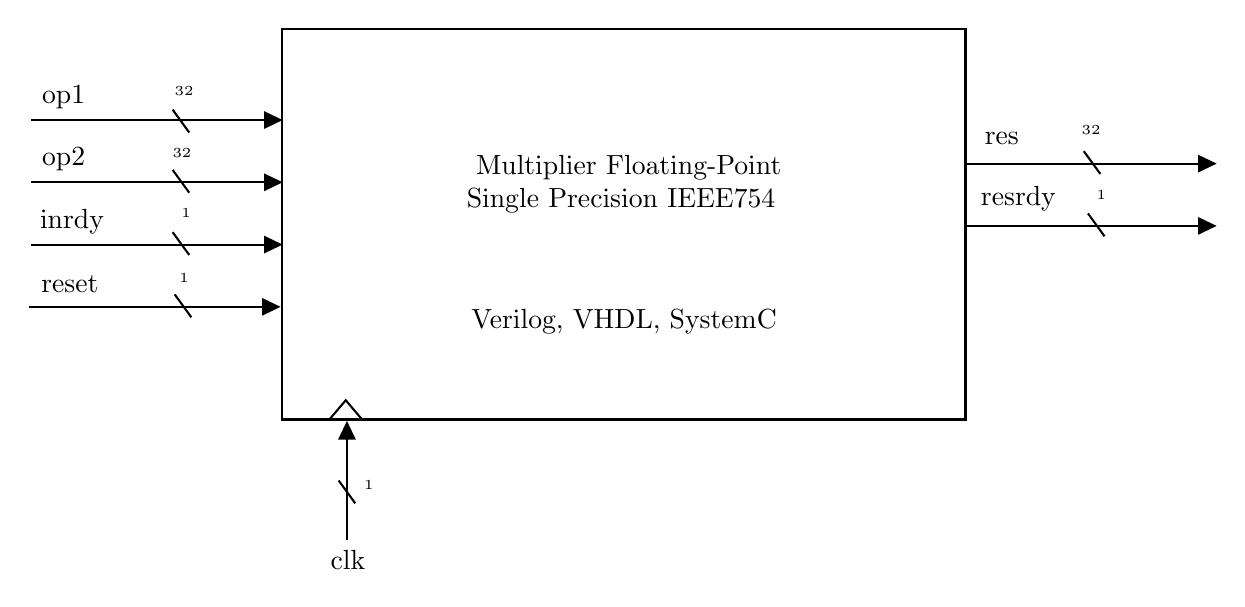
\begin{tikzpicture}[x=0.75pt,y=0.75pt,yscale=-1,xscale=1]
	%uncomment if require: \path (0,406); %set diagram left start at 0, and has height of 406
	
	%Shape: Rectangle [id:dp9211023518838333] 
	\draw   (165,86) -- (494.5,86) -- (494.5,274.29) -- (165,274.29) -- cycle ;
	%Straight Lines [id:da9591337699307748] 
	\draw    (44.17,130) -- (162.5,130) ;
	\draw [shift={(165.5,130)}, rotate = 180] [fill={rgb, 255:red, 0; green, 0; blue, 0 }  ][line width=0.08]  [draw opacity=0] (8.93,-4.29) -- (0,0) -- (8.93,4.29) -- cycle    ;
	
	%Straight Lines [id:da579702478769955] 
	\draw    (44.17,160) -- (162.5,160) ;
	\draw [shift={(165.5,160)}, rotate = 180] [fill={rgb, 255:red, 0; green, 0; blue, 0 }  ][line width=0.08]  [draw opacity=0] (8.93,-4.29) -- (0,0) -- (8.93,4.29) -- cycle    ;
	
	%Straight Lines [id:da76113659482319] 
	\draw    (44.17,190) -- (162.5,190) ;
	\draw [shift={(165.5,190)}, rotate = 180] [fill={rgb, 255:red, 0; green, 0; blue, 0 }  ][line width=0.08]  [draw opacity=0] (8.93,-4.29) -- (0,0) -- (8.93,4.29) -- cycle    ;
	
	%Straight Lines [id:da45600723803220433] 
	\draw    (43.17,220) -- (161.5,220) ;
	\draw [shift={(164.5,220)}, rotate = 180] [fill={rgb, 255:red, 0; green, 0; blue, 0 }  ][line width=0.08]  [draw opacity=0] (8.93,-4.29) -- (0,0) -- (8.93,4.29) -- cycle    ;
	
	%Straight Lines [id:da9181879524908487] 
	\draw    (494.17,151) -- (612.5,151) ;
	\draw [shift={(615.5,151)}, rotate = 180] [fill={rgb, 255:red, 0; green, 0; blue, 0 }  ][line width=0.08]  [draw opacity=0] (8.93,-4.29) -- (0,0) -- (8.93,4.29) -- cycle    ;
	
	%Straight Lines [id:da7910328097566827] 
	\draw    (494.17,181) -- (612.5,181) ;
	\draw [shift={(615.5,181)}, rotate = 180] [fill={rgb, 255:red, 0; green, 0; blue, 0 }  ][line width=0.08]  [draw opacity=0] (8.93,-4.29) -- (0,0) -- (8.93,4.29) -- cycle    ;
	
	%Shape: Triangle [id:dp124533916535147] 
	\draw   (195.92,265) -- (203.83,274.33) -- (188,274.33) -- cycle ;
	%Straight Lines [id:da309296107434495] 
	\draw    (196.5,332.33) -- (196.5,278) ;
	\draw [shift={(196.5,275)}, rotate = 450] [fill={rgb, 255:red, 0; green, 0; blue, 0 }  ][line width=0.08]  [draw opacity=0] (8.93,-4.29) -- (0,0) -- (8.93,4.29) -- cycle    ;
	
	%Straight Lines [id:da1421875224201805] 
	\draw    (112.5,125) -- (120.5,136) ;
	
	
	%Straight Lines [id:da13538438410660247] 
	\draw    (112.5,154) -- (120.5,165) ;
	
	
	%Straight Lines [id:da5317963116700639] 
	\draw    (112.5,184) -- (120.5,195) ;
	
	
	%Straight Lines [id:da8132393230886649] 
	\draw    (113.5,214) -- (121.5,225) ;
	
	
	%Straight Lines [id:da7586641121884944] 
	\draw    (192.5,303.67) -- (200.5,314.67) ;
	
	
	%Straight Lines [id:da33268972261161966] 
	\draw    (551.5,145) -- (559.5,156) ;
	
	
	%Straight Lines [id:da15050698861885248] 
	\draw    (553.5,175) -- (561.5,186) ;
	
	
	
	% Text Node
	\draw (330,161) node   [align=left] { \ Multiplier Floating-Point \\Single Precision IEEE754};
	% Text Node
	\draw (330,227) node   [align=left] {Verilog, VHDL, SystemC};
	% Text Node
	\draw (60,119) node   [align=left] {op1};
	% Text Node
	\draw (60,149) node   [align=left] {op2};
	% Text Node
	\draw (64,179) node   [align=left] {inrdy};
	% Text Node
	\draw (63,209) node   [align=left] {reset};
	% Text Node
	\draw (197,342) node   [align=left] {clk};
	% Text Node
	\draw (512,139) node   [align=left] {res};
	% Text Node
	\draw (520,168) node   [align=left] {resrdy};
	% Text Node
	\draw (555,135) node   [align=left] {{\tiny 32}};
	% Text Node
	\draw (560,166) node   [align=left] {{\tiny 1}};
	% Text Node
	\draw (207,306) node   [align=left] {{\tiny 1}};
	% Text Node
	\draw (118,206) node   [align=left] {{\tiny 1}};
	% Text Node
	\draw (119,175) node   [align=left] {{\tiny 1}};
	% Text Node
	\draw (117,146) node   [align=left] {{\tiny 32}};
	% Text Node
	\draw (118,116) node   [align=left] {{\tiny 32}};
	
		\end{tikzpicture}